\documentclass{article}
\title{The application of noisy-channel coding techniques to DNA barcoding}
\author{\begin{tabular}{rl}
        Name:& Izaak van Dongen\\
        EP Mentor:& Nicolle Mcnaughton\\
        Tutor:& Paul Ingham\\
        Candidate No:&  6659\\
        \end{tabular}
        }

% make the document take up more of the page
\usepackage{fullpage}

% pretty table rules and multirow entries
\usepackage{booktabs}
\usepackage{multirow}

% plotting mathematical functions (needs version request)
\usepackage{pgfplots}
\pgfplotsset{compat=1.15}

% \url function and clickable table of contents
\usepackage[hidelinks]{hyperref}

% maths symbols
\usepackage{amsmath}
\usepackage{amsfonts}
\usepackage{amssymb}
\usepackage{commath}

% courier font
\usepackage{courier}

% bibliography in table of contents, correctly.
\usepackage[nottoc]{tocbibind}

% no paragraph indent
\usepackage[parfill]{parskip}

% more advanced handling of utf8 and fonts
\usepackage[utf8]{inputenc}
\usepackage[T1]{fontenc}

% bibliography management
\usepackage[square]{natbib}

% graphics, like postscript
\usepackage{graphicx}

% used to horizontally align floats
\usepackage{subfig}

% used for figures
\usepackage{float}

% code listings
\usepackage{listings}

% needed for code listings and colouring
\usepackage{color}

\definecolor{codegreen}{rgb}{ 0,0.6,0}
\definecolor{codegray}{rgb}{0.5,0.5,0.5}
\definecolor{codepurple}{rgb}{0.58,0,0.82}
\definecolor{backcolour}{rgb}{0.95,0.95,0.92}

% listing style
\lstdefinestyle{mystyle}{
    backgroundcolor=\color{backcolour},
    commentstyle=\color{codegreen},
    keywordstyle=\color{magenta},
    numberstyle=\tiny\color{codegray},
    stringstyle=\color{codepurple},
    basicstyle=\footnotesize,
    breaklines=true,
    postbreak=\mbox{\textcolor{red}{$\hookrightarrow$}\space},
    captionpos=b,
    keepspaces=true,
    numbers=left,
    numbersep=5pt,
    showspaces=false,
    showstringspaces=false,
    showtabs=false,
    tabsize=2
}

\lstset{style=mystyle}

% listing exceptionsal characters
\lstset{
    literate={~} {$\sim$}{1}
}

% stop things from jumping across to pages too much.
\allowdisplaybreaks

\begin{document}
    \maketitle
    \tableofcontents
    \lstlistoflistings
    \listoffigures
    \listoftables

    \section{Introduction}
    The premise of this project is to investigate the different types of
    error-correcting codes, and how these might be applied to DNA barcoding.
    The challenge in this comes from the fact that most error-correcting codes
    are designed in base-2 (binary) whereas DNA strings are fundamentally
    base-4 (quaternary). The applicability of this project is that in
    oligonucleotide synthesis, some samples may need to be identified later on
    using a subsection of the sample (a barcode). These could just be linearly
    assigned codes, but this would leave them very susceptible to mutation.

    Here is an example: say that we're given a barcode of length four, to
    encode two different samples. If we worked methodically up from the bottom
    (using the ordering ACGT - orderings will be discussed further later on) we
    might end up with the codes AAAA and AAAC. However, either string would
    only require a single mutation (where we say a mutation is the changing of
    a single base) to become identical to the other one. Therefore, in this
    case, it would clearly be far more optimal to make a choice like, for
    example, AAAA and CCCC.

    There have been a few assumptions and glossed over definitions here:

    \begin{itemize}
        \item What constitutes a mutation?
        \item What is the best way to represent DNA mathematically?
    \end{itemize}

    There are also a number of parameters to the problem, and as they change
    the problem becomes very much nontrivial:

    \begin{itemize}
    \item What if the barcode size changes?
    \item What if we want more codes than two?
    \item What if rather than number of codes and barcode size, the parameters
          are set to barcode size and maximum number of mutations that can
          occur?
    \end{itemize}

    All of these will be further explored in this dissertation.

    Note that I have written various ``scripts'', or ``programs''. These are
    basically a series of instructions written in a certain programming
    ``language'' that tell the computer what to do. When these are included the
    the dissertation, they will generally also have ``comments'' in them. These
    are sections of the code which are preceded by a special character (normally
    \% or \#) that tells the computer to ignore these. The comments should be
    highlighted in green. They will offer a simplified explanation of what the
    code does.

    \section{The Hamming distance}

    The Hamming distance is a measure of ``string distance''. String
    distance is a way to define how different two string are.
    Coding-theoretically, this can be used to quantify the amount that a
    string has been changed by transmission (or an oligonucleotide has been
    mutated).

    The Hamming distance between any two equally long strings $S$ and $R$
    is given by the number of characters at identical position that differ.
    For example, if we let $d_H$ denote Hamming distance, the distances
    \begin{align*}
    d_H(S, R) &= 1\\
    d_H(S, T) &= 2\\
    \text{where}\
    S &= \texttt{abcde}\\
    R &= \texttt{abc\textcolor{blue}{f}e}\\
    T &= \texttt{a\textcolor{codegreen}{x}c\textcolor{codegreen}{z}e}
    \end{align*}
    Note that for any $S$, $d(S, S) = 0$. This means that there is no
    ``distance'' from a string to itself.

    In terms of DNA, the Hamming distance can be used to determine the
    number of bases that have mutated.

%TODO citation needed

    \section{Parity codes}

    The insertion of ``parity bits'' is a common practice in basic encoding.
    Parity refers to the ``oddness'' or ``evenness'' of some data. Commonly,
    this is determined by the sum of the data modulo 2. For example, ``00101''
    results in a parity bit of 0, because the sum of all the bits is 2, which
    has a remainder of 0 when divided by 2 (is equal to 0 mod 2).

    A simple but inefficient parity encoding scheme is a column/row wise
    encoding. Take the slightly contrived data string ``0100000101010100''.
    This is very tangentially related to DNA - it's the 8-bit ASCII
    representation of the string ``AT'', generated by the Python:
    \lstinline[language=Python]|"". join(bin(ord(c))[2:].rjust(8, "0") for c in "AT")|

%TODO cite ASCII

    The string is then split into a square like so:

    \begin{center}
    \begin{math}
    \begin{matrix}
        0 & 1 & 0 & 0 \\
        0 & 0 & 0 & 1 \\
        0 & 1 & 0 & 1 \\
        0 & 1 & 0 & 0
    \end{matrix}
    \end{math}
    \end{center}

    An extra row and column, including an extra corner piece is appended like
    so:

    \begin{center}
    \begin{tabular}{c c c c | c}
        0 & 1 & 0 & 0 & 1 \\
        0 & 0 & 0 & 1 & 1 \\
        0 & 1 & 0 & 1 & 0 \\
        0 & 1 & 0 & 0 & 1 \\ \hline
        0 & 1 & 0 & 0 & 1
   \end{tabular}
   \end{center}

   Each of the extra bits documents the pairty of its row. Using a scheme like
   this, a single corrupted bit can be detected, and corrected. For example,
   the bit at (3, 4) may have flipped like so:

    \begin{center}
    \begin{tabular}{c c c c | c}
        0 & 1 & 0 & 0 & 1 \\
        0 & 0 & 0 & 1 & 1 \\
        0 & 1 & 0 & 1 & 0 \\
        0 & 1 & \textcolor{red}{1} & 0 & 1 \\ \hline
        0 & 1 & 0 & 0 & 1
   \end{tabular}
   \end{center}

    Someone wishing to correct this error can check the parity of each column,
    compared with its parity bit. They can do the same for each row. Assuming
    one error has occurred, the point where the incorrect row and column cross
    is to be flipped back. In this case, the third column doesn't add up, and
    the fourth row doesn't add up, leading to the faulty bit. It is worth
    noting that this also works to correct errors in the parity bits, due the
    the extra corner bit. If only the extra corner bit seems to be wrong, it is
    the one that has flipped.

    However, this particularly scheme is in a sense quite inefficient. At the
    most optimal configuration, it uses on the order of $2\sqrt{n}$ parity bits,
    where $n$ is the number of bits in the message, in order to achieve 1
    correction. This can be proven as follows:

    Assume $n$ to be highly divisible. Let $p$ denote the number of parity
    bits, and $x$ denote the length of a row. We then have,

    \begin{align*}
        p &= \frac{n}{x} + x \\
        \Rightarrow \frac{dp}{dx} &= 1 - \frac{n}{x^2}
                    = 0\ \text{(as $p$ must be a minimum)}\\
        \Rightarrow 1 &= \frac{n}{x^2} \\
        \Rightarrow x^2 &= n \\
        \Rightarrow x &= \sqrt{n} \\
        \Rightarrow p &= \frac{n}{\sqrt{n}} + \sqrt{n} = \sqrt{n} + \sqrt{n} \\
                      &= 2\sqrt{n} \\
    \end{align*}

    This is quite a poor asymptotic performance - as the number of data bits
    grows larger, the number of parity bits required grows relatively fast. In
    the next section, I describe a similar code that uses only $\log_2 n$. Here
    is a quick plot comparing the two functions:

\begin{center}
    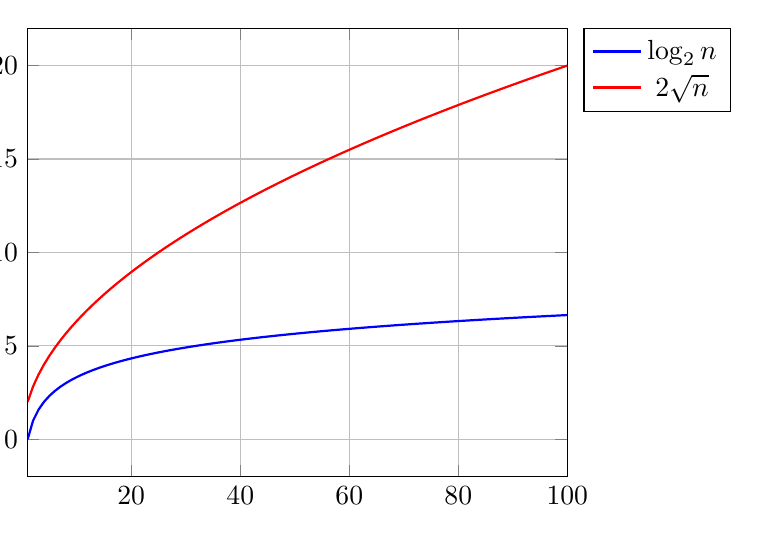
\begin{tikzpicture}[trim axis left]
    \begin{axis}[
      domain=1:100,
      no markers,
      samples=100,
      enlarge x limits=false,
      grid=both,
legend entries={$\log_2 n$,
                $2\sqrt{n}$},
legend pos=outer north east]
    \addplot +[thick] {ln(x)/ln(2)};
    \addplot +[thick] {2 * sqrt(x)};
    \end{axis}
    \end{tikzpicture}
\end{center}

    As you can see, as $n$ increases the relative performance of the row-column
    approach degrades significantly.

    \section{The Hamming code}

    The Hamming code instead places a parity bit at each index that is a power
    of two, where we number indices starting from 1. Therefore, our previous
    data string gains parity bits in this configuration:
    \textcolor{red}{10}0\textcolor{red}{1}100\textcolor{red}{0}0001010\textcolor{red}{0}10100
    (the 1st, 2nd, 4th, 8th and 16th bits are used for parity).

    The way the parity ``coverage'' works is shown in table
    \ref{tab:hamming-indices}.  I have included indices up to 31. This is
    because that is the longest encodable string with only five parity bits
    (afterwards, we have to add a parity bit at 32). Of course, a shorter code
    word can always also be encoded by just acting as if each index that is out
    of range is a 0.

\begin{table}[h]
\begin{center}
    \begin{tabular}{crrrrrrrrrrrrrrr}
    \toprule
    Parity index & \multicolumn{15}{c}{Covered indices} \\
    \midrule
    1 & 3 & 5 & 7 & 9 & 11 & 13 & 15 & 17 & 19 & 21 & 23 & 25 & 27 & 29 & 31 \\
    2 & 3 & 6 & 7 & 10 & 11 & 14 & 15 & 18 & 19 & 22 & 23 & 26 & 27 & 30 & 31 \\
    4 & 5 & 6 & 7 & 12 & 13 & 14 & 15 & 20 & 21 & 22 & 23 & 28 & 29 & 30 & 31 \\
    8 & 9 & 10 & 11 & 12 & 13 & 14 & 15 & 24 & 25 & 26 & 27 & 28 & 29 & 30 & 31 \\
    16 & 17 & 18 & 19 & 20 & 21 & 22 & 23 & 24 & 25 & 26 & 27 & 28 & 29 & 30 & 31 \\
    \bottomrule
    \end{tabular}
    \caption{Parity coverage in a Hamming code}\label{tab:hamming-indices}
\end{center}
\end{table}

    These are very deliberately chosen indices. In fact, this table was
    generated by a short code snippet that can be found in listing
    \ref{lst:hamtab}.

    The way that it works is by considering the value of the parity index in
    binary. For example, $4_{10}=100_{2}$. As they are powers of two, they will
    always be of the form `$10*$' (a one followed by 0 or more zeroes).

    The code in listings \ref{lst:hamcol} and \ref{lst:hamps} generates two
    visualisations, which I find helpful. The first is table
    \ref{tab:hamming-binary}, which is similar to table
    \ref{tab:hamming-indices}, but transposed so each column corresponds to a
    parity bit, and each index is written in binary:

\begin{table}[h]
\begin{center}
    \begin{tabular}{l|rrrrr}
    \toprule
    Parity index & \texttt{0000\textcolor{blue}{1}} & \texttt{000\textcolor{blue}{1}0} & \texttt{00\textcolor{blue}{1}00} & \texttt{0\textcolor{blue}{1}000} & \texttt{\textcolor{blue}{1}0000} \\
    \midrule
    \multirow{14}{*}{Coverage} & \texttt{0001\textcolor{blue}{1}} & \texttt{000\textcolor{blue}{1}1} & \texttt{00\textcolor{blue}{1}01} & \texttt{0\textcolor{blue}{1}001} & \texttt{\textcolor{blue}{1}0001} \\
    & \texttt{0010\textcolor{blue}{1}} & \texttt{001\textcolor{blue}{1}0} & \texttt{00\textcolor{blue}{1}10} & \texttt{0\textcolor{blue}{1}010} & \texttt{\textcolor{blue}{1}0010} \\
    & \texttt{0011\textcolor{blue}{1}} & \texttt{001\textcolor{blue}{1}1} & \texttt{00\textcolor{blue}{1}11} & \texttt{0\textcolor{blue}{1}011} & \texttt{\textcolor{blue}{1}0011} \\
    & \texttt{0100\textcolor{blue}{1}} & \texttt{010\textcolor{blue}{1}0} & \texttt{01\textcolor{blue}{1}00} & \texttt{0\textcolor{blue}{1}100} & \texttt{\textcolor{blue}{1}0100} \\
    & \texttt{0101\textcolor{blue}{1}} & \texttt{010\textcolor{blue}{1}1} & \texttt{01\textcolor{blue}{1}01} & \texttt{0\textcolor{blue}{1}101} & \texttt{\textcolor{blue}{1}0101} \\
    & \texttt{0110\textcolor{blue}{1}} & \texttt{011\textcolor{blue}{1}0} & \texttt{01\textcolor{blue}{1}10} & \texttt{0\textcolor{blue}{1}110} & \texttt{\textcolor{blue}{1}0110} \\
    & \texttt{0111\textcolor{blue}{1}} & \texttt{011\textcolor{blue}{1}1} & \texttt{01\textcolor{blue}{1}11} & \texttt{0\textcolor{blue}{1}111} & \texttt{\textcolor{blue}{1}0111} \\
    & \texttt{1000\textcolor{blue}{1}} & \texttt{100\textcolor{blue}{1}0} & \texttt{10\textcolor{blue}{1}00} & \texttt{1\textcolor{blue}{1}000} & \texttt{\textcolor{blue}{1}1000} \\
    & \texttt{1001\textcolor{blue}{1}} & \texttt{100\textcolor{blue}{1}1} & \texttt{10\textcolor{blue}{1}01} & \texttt{1\textcolor{blue}{1}001} & \texttt{\textcolor{blue}{1}1001} \\
    & \texttt{1010\textcolor{blue}{1}} & \texttt{101\textcolor{blue}{1}0} & \texttt{10\textcolor{blue}{1}10} & \texttt{1\textcolor{blue}{1}010} & \texttt{\textcolor{blue}{1}1010} \\
    & \texttt{1011\textcolor{blue}{1}} & \texttt{101\textcolor{blue}{1}1} & \texttt{10\textcolor{blue}{1}11} & \texttt{1\textcolor{blue}{1}011} & \texttt{\textcolor{blue}{1}1011} \\
    & \texttt{1100\textcolor{blue}{1}} & \texttt{110\textcolor{blue}{1}0} & \texttt{11\textcolor{blue}{1}00} & \texttt{1\textcolor{blue}{1}100} & \texttt{\textcolor{blue}{1}1100} \\
    & \texttt{1101\textcolor{blue}{1}} & \texttt{110\textcolor{blue}{1}1} & \texttt{11\textcolor{blue}{1}01} & \texttt{1\textcolor{blue}{1}101} & \texttt{\textcolor{blue}{1}1101} \\
    & \texttt{1110\textcolor{blue}{1}} & \texttt{111\textcolor{blue}{1}0} & \texttt{11\textcolor{blue}{1}10} & \texttt{1\textcolor{blue}{1}110} & \texttt{\textcolor{blue}{1}1110} \\
    & \texttt{1111\textcolor{blue}{1}} & \texttt{111\textcolor{blue}{1}1} & \texttt{11\textcolor{blue}{1}11} & \texttt{1\textcolor{blue}{1}111} & \texttt{\textcolor{blue}{1}1111} \\
    \bottomrule
    \end{tabular}
    \caption{Indices covered by each parity bit shown in binary}\label{tab:hamming-binary}
\end{center}
\end{table}

    The second is shown in Figure \ref{fig:hamming}. It represents each covered
    bit as a filled in square, and each non-covered bit as an empty square, so
    the whole codeword is shown in every row.

\begin{figure}[h]
\begin{center}
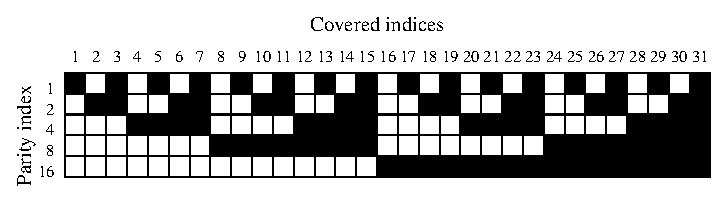
\includegraphics{../psfiles/hamming_visualisation.eps}
\end{center}
\caption{Index coverage of Hamming parity bits}\label{fig:hamming}
\end{figure}

    The script implementing a simple binary Hamming code is as follows:

\lstinputlisting[language=Python, caption=Binary Hamming code in Python]
{../src/binary_hamming.py}

    This code is accompanied by the following testing scheme:

\lstinputlisting[language=Python, caption=binary\_hamming unit tests]
{../src/test_binary_hamming.py}

    \section{Adapting the Hamming code}

    Unfortunately, this all only operates on binary data, as this is more of a
    `fundamental' base.. As is, this is of no use because DNA strings are
    fundamentally base-4.

    \section{The Hadamard code}

%TODO citations, maybe hedayat

    The Hadamard code is based on Hadamard matrices. A Hadamard matrix is a
    matrix such that each pair of rows represent a pair of orthogonal vectors.
    Practically, this means that each row has a Hamming distance of at least
    half of its length from each other row. This is a much stronger encoding
    than the Hamming code, so may be much more resistant to mutations. However,
    as a natural side effect of this, Hadamard codes are longer and more sparse.

    Here is the code implementing the basic $2^n$ hadamard matrix generation
    scheme:

\lstinputlisting[language=Python, caption=Hadamard matrix generation]
{../src/hadamard_matrix.py}

%TODO talk about sphere packing

%TODO add mindmap

    A visualistion of the Hadamard matrix is provided by the Python script in
    listing \ref{lst:hadpy}. It displays the matrix as a grid, where each `1' is
    filled in, as in figure \ref{fig:hadvis}.

\begin{figure}[h]
\begin{center}
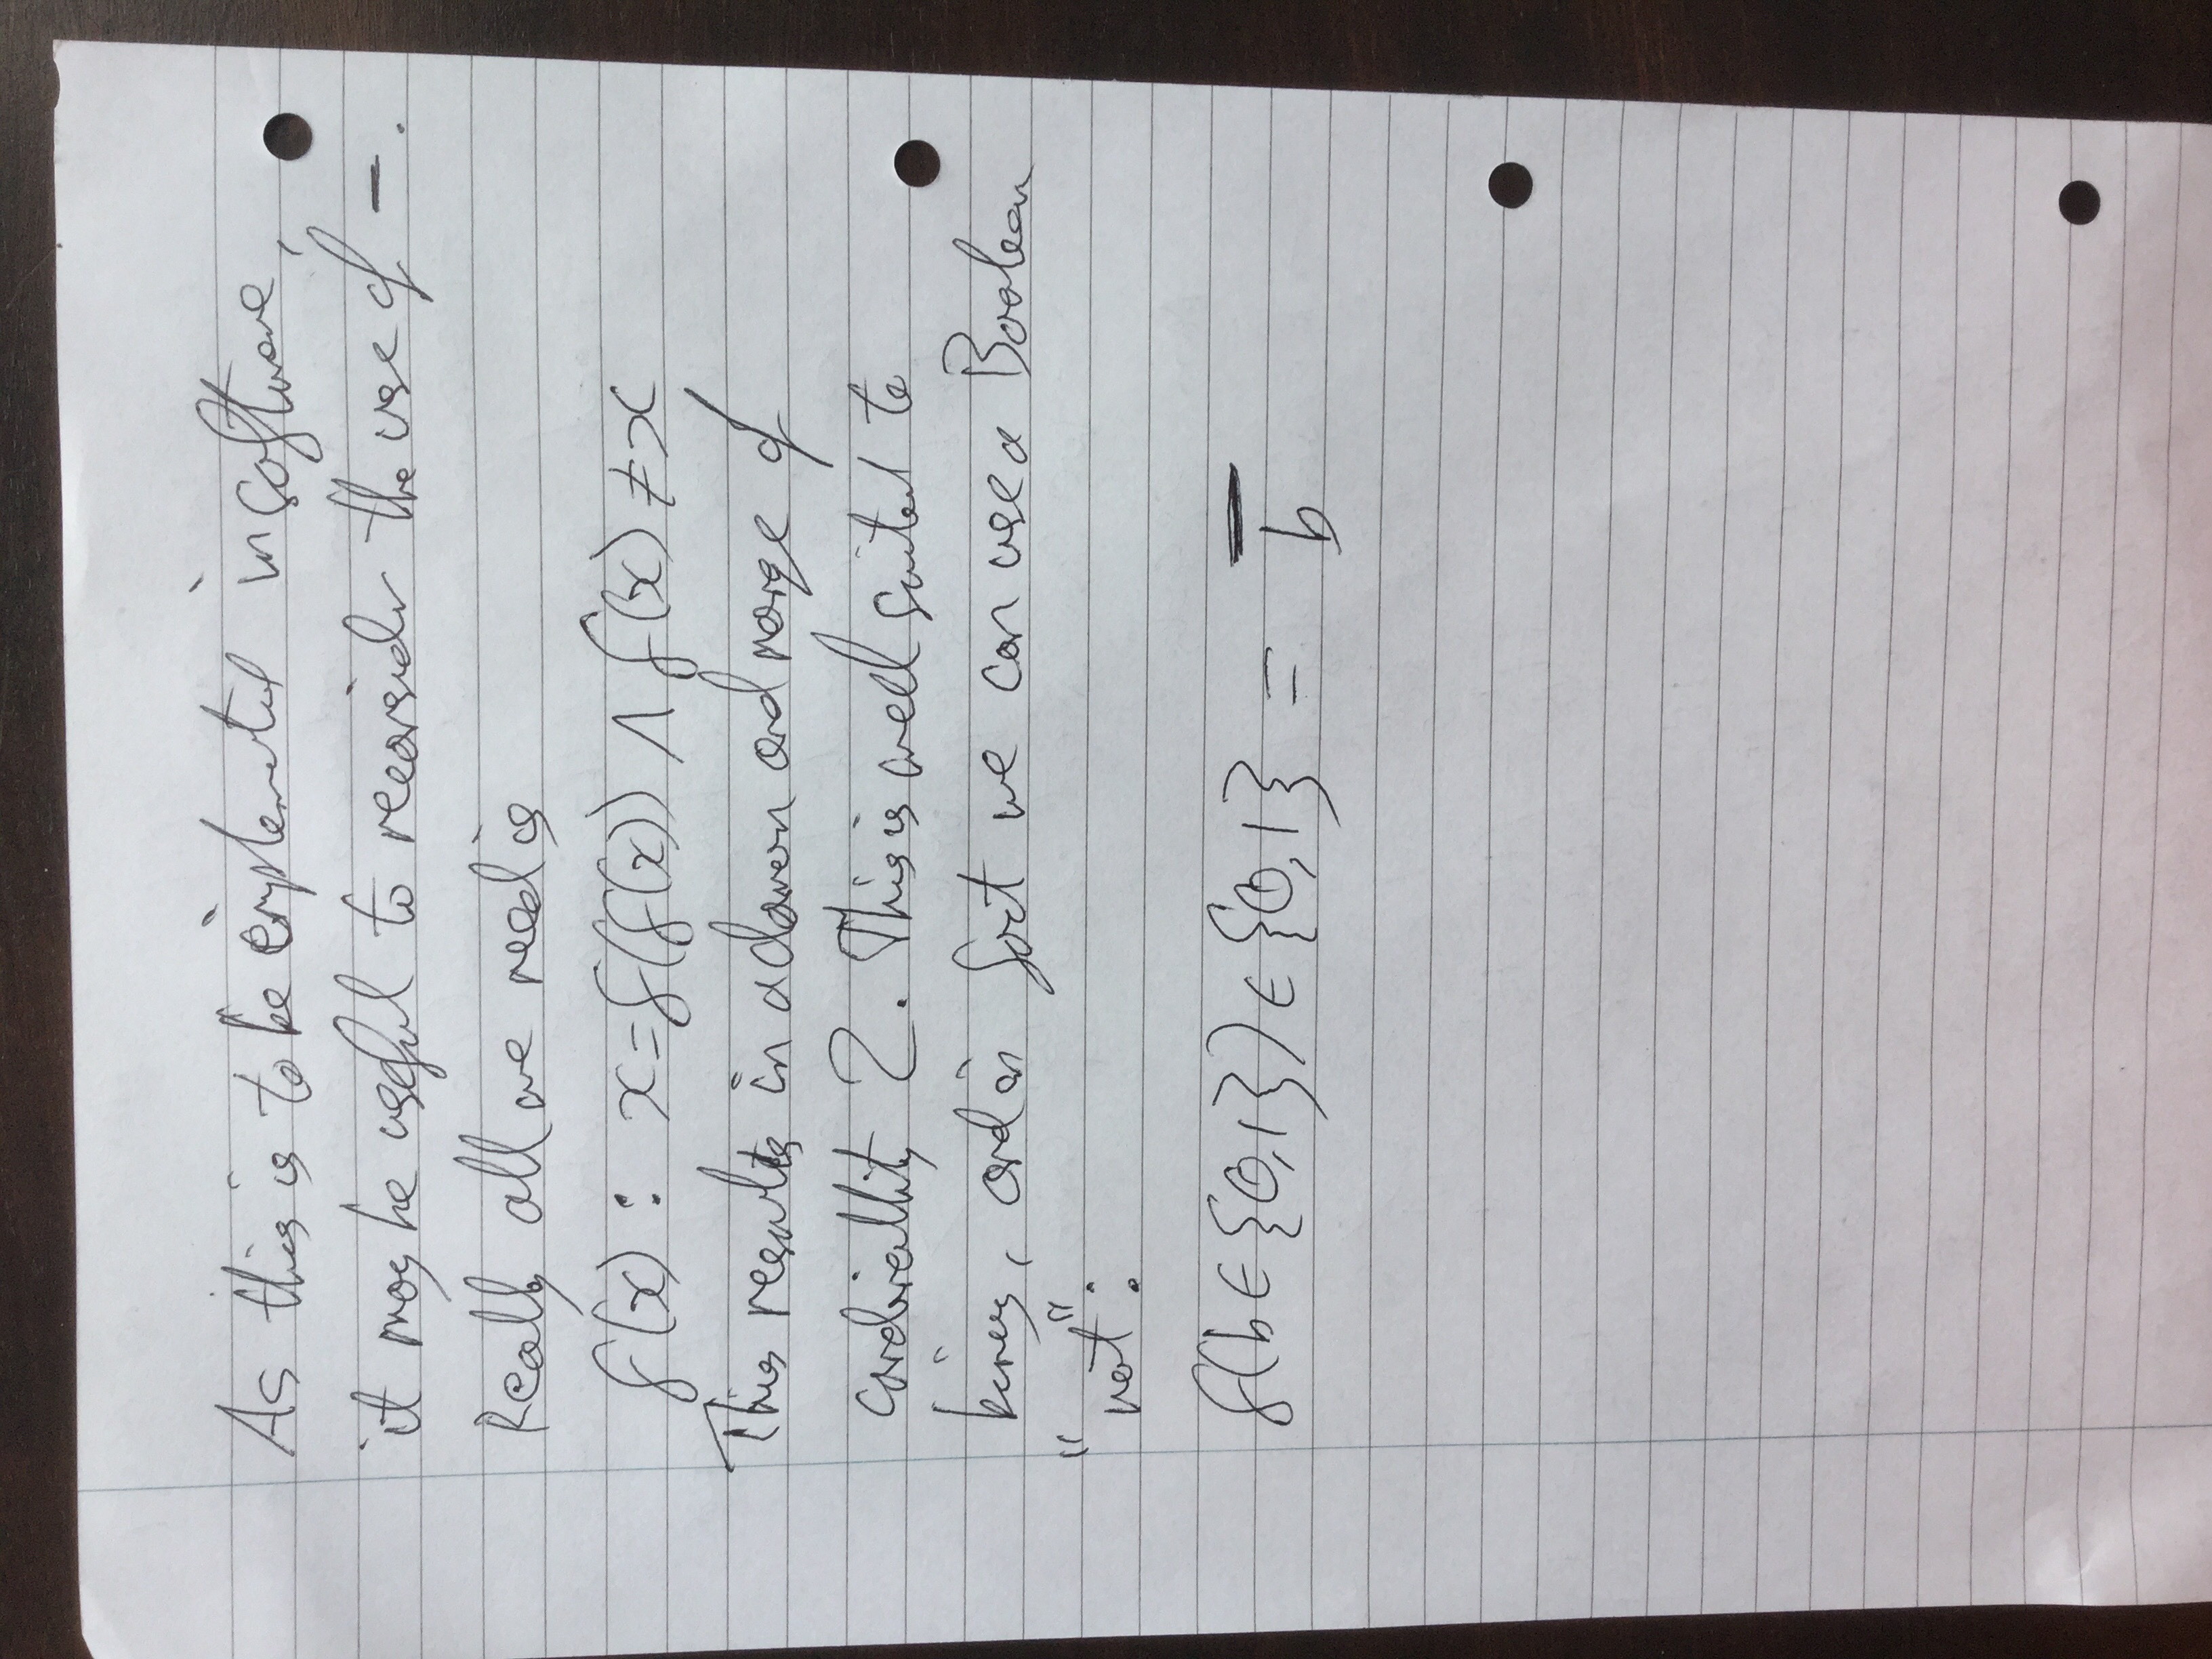
\includegraphics[height=0.3\textheight]{../psfiles/hadamard_2.eps}%
\hfill%

\includegraphics[height=0.3\textheight]{../psfiles/hadamard_3.eps}%
\hfill%
\includegraphics[height=0.3\textheight]{../psfiles/hadamard_4.eps}%
\hfill%
\includegraphics[height=0.3\textheight]{../psfiles/hadamard_5.eps}%
\end{center}
\caption{Visualisation of ``$2^n$'' Hadamard matrices}\label{fig:hadvis}
\end{figure}

    \section{Unit tests}

    For all the core programs, I have also written unit tests. These aim to
    verify that the program works by presenting a number of test cases, and
    seeing if the program produces the correct output. These both help to ensure
    correct behaviour, and can serve as a more practical reference of how I
    expect functions to behave.

\lstinputlisting[language=Python, caption=Unit tests for binary\_hamming]
{../src/test_binary_hamming.py}

    \section{Miscellaneous listings}

\begin{lstlisting}[language=Python, caption=Generating Hamming coverage indices,
                   label=lst:hamtab]
for p_ind in (1 << pwr for pwr in range(5)):
    print(r"    {} \\".format(" & ".join(str(i) for i in range(1, 33) if i & p_ind)))
\end{lstlisting}

\begin{lstlisting}[language=Python, caption=Generating binary table,
                   label={lst:hamcol}]
def add_color(s, ind):
    return r"{}\textcolor{{blue}}{{{}}}{}".format(s[:ind], s[ind], s[ind+1:])

table = zip(*[[i for i in range(1, 33) if i & p_ind] for p_ind in (1 << pwr for pwr in range(5))])
print("\n".join(r"    {} \\".format(" & ".join(r"\texttt{{{}}}".format(add_color(bin(i)[2:].rjust(5, "0"), 4 -sig_ind))
            for sig_ind, i in enumerate(row)))
            for row in table))
\end{lstlisting}

\lstinputlisting[language=Postscript, caption=Hamming index coverage,
                 label={lst:hamps}]
{../psfiles/hamming_visualisation.ps}

\lstinputlisting[language=Python,
                 caption=Hadamard visualisation (uses code in \ref{lst:hadps}),
                 label={lst:hadpy}]
{../src/generate_ham_vis.py}

\lstinputlisting[language=Postscript, caption=Template for Hadamard graphic,
                 label={lst:hadps}]
{../src/hadamard_template.ps}

    \section{Source}

    This document consists of about
    \input{|"texcount dissertation.tex | awk '/^Words in text/{print $NF-1}'"}
    words.

    All code and source \TeX/\LaTeX{} files can be found at
    \url{https://github.com/elterminad0r/EPQ}.

%TODO classifications of codes by number of correctable errors

\nocite{*}

\bibliographystyle{agsm}
\bibliography{sources}

\end{document}
